\hypertarget{modelview2_8cpp}{}\section{Файл Projects/labs/course\+\_\+project\+\_\+cg/src/widgets/modelview2.cpp}
\label{modelview2_8cpp}\index{Projects/labs/course\+\_\+project\+\_\+cg/src/widgets/modelview2.\+cpp@{Projects/labs/course\+\_\+project\+\_\+cg/src/widgets/modelview2.\+cpp}}
{\ttfamily \#include \char`\"{}modelview2.\+h\char`\"{}}\\*
{\ttfamily \#include \char`\"{}src/animation/rotatetransformation.\+h\char`\"{}}\\*
{\ttfamily \#include \char`\"{}src/animation/scene.\+h\char`\"{}}\\*
{\ttfamily \#include \char`\"{}src/animation/renderer.\+h\char`\"{}}\\*
{\ttfamily \#include \char`\"{}src/animation/sceneobjectfactory.\+h\char`\"{}}\\*
{\ttfamily \#include \char`\"{}src/animation/lightzbufferrenderer.\+h\char`\"{}}\\*
{\ttfamily \#include \char`\"{}src/animation/objloader.\+h\char`\"{}}\\*
{\ttfamily \#include \char`\"{}src/animation/scaletransformation.\+h\char`\"{}}\\*
{\ttfamily \#include \char`\"{}src/animation/movetransformation.\+h\char`\"{}}\\*
{\ttfamily \#include \char`\"{}src/animation/actions.\+h\char`\"{}}\\*
{\ttfamily \#include $<$Q\+Painter$>$}\\*
Граф включаемых заголовочных файлов для modelview2.\+cpp\+:\nopagebreak
\begin{figure}[H]
\begin{center}
\leavevmode
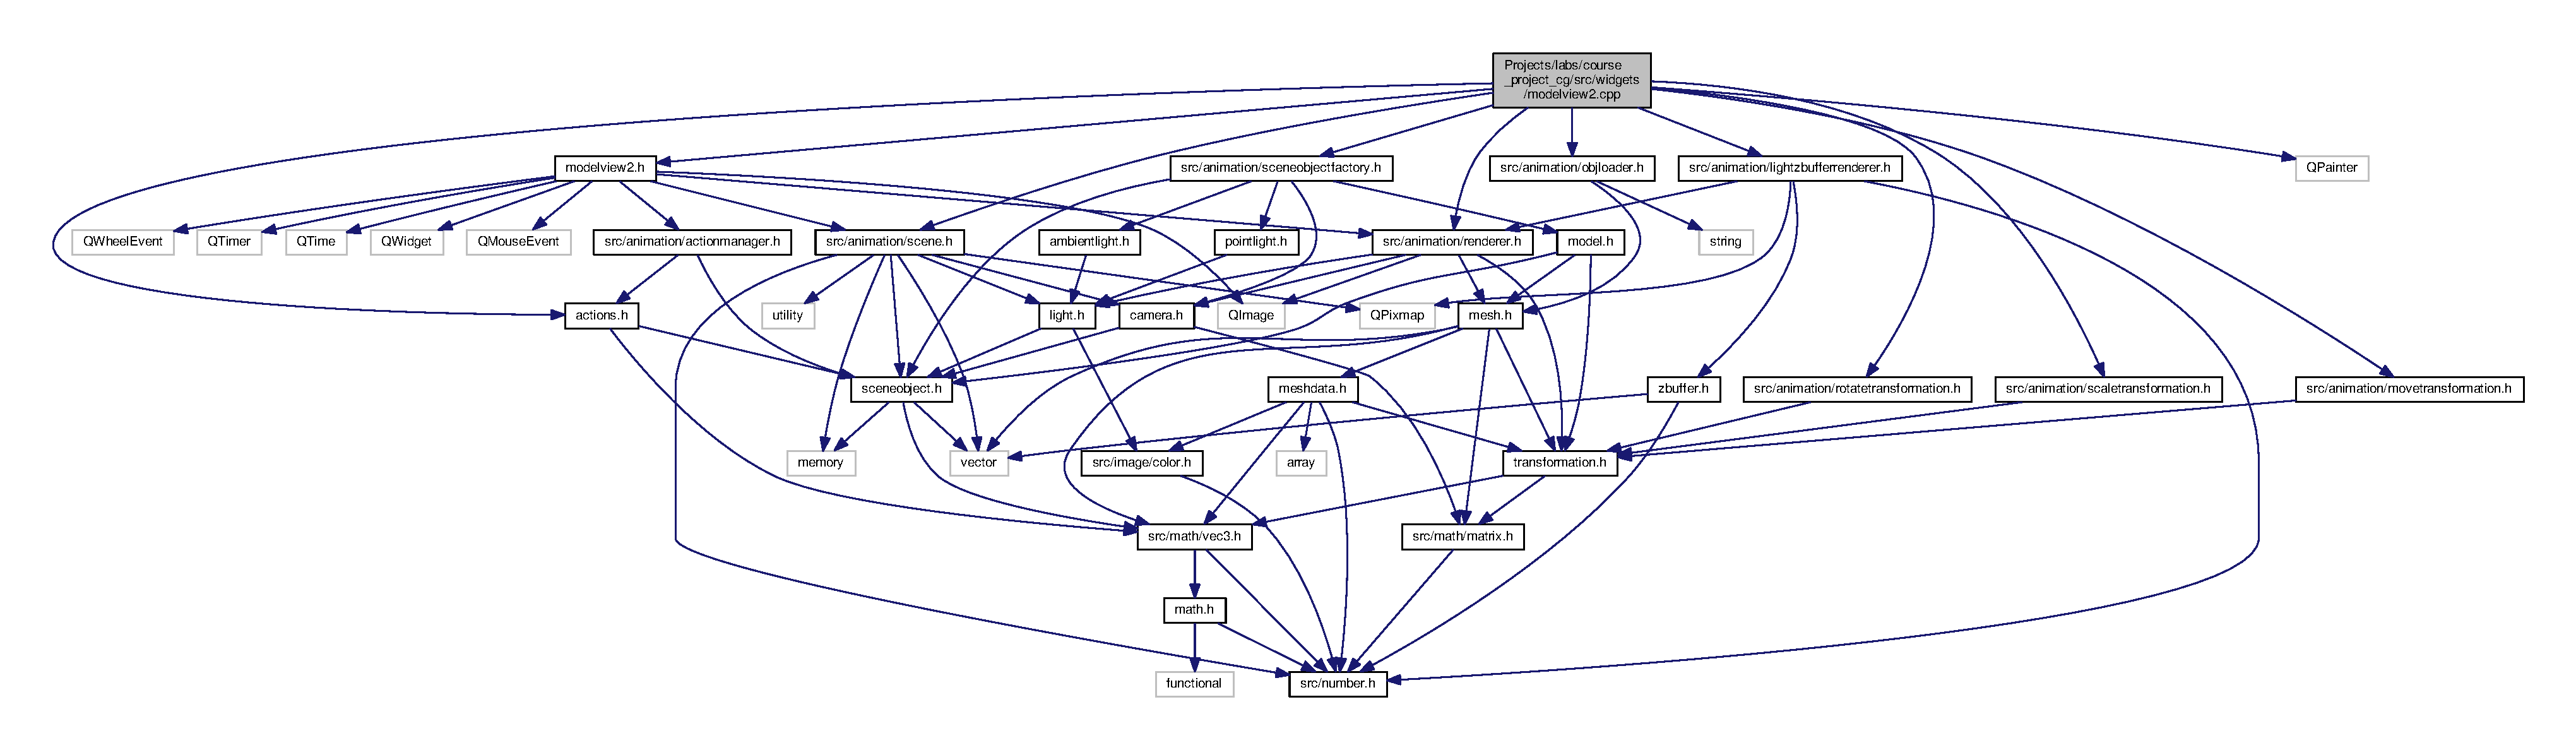
\includegraphics[width=350pt]{d6/da0/modelview2_8cpp__incl}
\end{center}
\end{figure}
